% ------------------------------------------------------------------------------
% Centro Federal de Educação Tecnológica de Minas Gerais - CEFET-MG
%
% Modelo de trabalho acadêmico em conformidade com as normas da ABNT
% (Tese de Doutorado, Dissertação de Mestrado ou Projeto de Qualificação)
%
% Projeto hospedado em: https://github.com/cfgnunes/latex-cefetmg
%
% Autores: Cristiano Nunes <cfgnunes@gmail.com>
%          Henrique Borges <henrique@cefetmg.br>
% ------------------------------------------------------------------------------

\documentclass[oneside]{cefetmg}    % Impressão apenas no anverso
%\documentclass[twoside]{cefetmg}   % Impressão em frente (anverso) e verso

% ------------------------------------------------------------------------------
% Pacotes utilizados
% ------------------------------------------------------------------------------
\usepackage[utf8]{inputenc}         % Codificação do documento
\usepackage[T1]{fontenc}            % Seleção de código de fonte
\usepackage{booktabs}               % Réguas horizontais em tabelas
\usepackage{color, colortbl}        % Controle de cores
\usepackage{float}                  % Tabelas/figuras em ambiente multicolunas
\usepackage{graphicx}               % Inclusão de gráficos
\usepackage{icomma}                 % Uso de vírgulas em expressões matemáticas
\usepackage{indentfirst}            % Recua o primeiro parágrafo de cada seção
\usepackage{microtype}              % Melhora a justificação do documento
\usepackage{multirow, makecell}     % Tabelas com múltiplas linhas e colunas
\usepackage{subeqnarray}            % Subenumeração de equações
\usepackage{verbatim}               % Exibir texto tal como escrito no documento
\usepackage{amsmath}                % Fontes e símbolos matemáticos
\usepackage{xfrac}                  % Escrever frações de forma compacta
\usepackage[charter]{mathdesign}    % Utiliza a fonte Charter BT
%\usepackage{times}                 % Utiliza a fonte Times
%\usepackage{newtxtext,newtxmath}   % Utiliza a fonte Times (melhorado)
%\usepackage{palatino}              % Utiliza a fonte Palatino
%\usepackage{latexsym}              % Símbolos matemáticos
%\usepackage{lscape}                % Páginas em modo paisagem

% Utiliza a fonte Helvetica (similar a fonte Arial)
%\usepackage{helvet}
%\renewcommand*\familydefault{\sfdefault}

% ------------------------------------------------------------------------------
% Configurações de aparência do PDF final
% ------------------------------------------------------------------------------

% Define a cor utilizada nos links do PDF
\definecolor{blue_link}{RGB}{0,80,128}

% Configuração dos metadados do PDF (palavras-chave)
\hypersetup{pdfkeywords={%
    Palavra-chave 1, Palavra-chave 2, Palavra-chave 3, Palavra-chave 4.
}}

% Hifenização de palavras que não estão no dicionário
%\hyphenation{%
%    qua-dros-cha-ve
%    Kat-sa-gge-los
%}

% ------------------------------------------------------------------------------
% Inclui os arquivos do trabalho acadêmico
% ------------------------------------------------------------------------------

% Insere alguns elementos para gerar capa, folha de rosto e folha de aprovação
% ------------------------------------------------------------------------------
% Dados do trabalho acadêmico
% ------------------------------------------------------------------------------

\titulo{Título do Trabalho}
%\title{Title in English}
\subtitulo{Subtítulo do trabalho}
\autor{Nome completo do autor}
\local{Belo Horizonte}
\data{Maio de 2021} % Normalmente se usa apenas mês e ano

% ------------------------------------------------------------------------------
% Natureza do trabalho acadêmico
% Use apenas uma das opções: Tese (p/ Doutorado), Dissertação (p/ Mestrado) ou
% Projeto de Qualificação (p/ Mestrado ou Doutorado), Trabalho de Conclusão de
% Curso (Graduação)
% ------------------------------------------------------------------------------

\projeto{Projeto de Qualificação}

% ------------------------------------------------------------------------------
% Título acadêmico
% Use apenas uma das opções:
% - Se a natureza for Tese, coloque Doutor
% - Se a natureza for Dissertação, coloque Mestre
% - Se a natureza for Projeto de Qualificação, coloque Mestre ou Doutor
% - Se a natureza for Trabalho de Conclusão de Curso, coloque Bacharel
% ------------------------------------------------------------------------------

\tituloAcademico{Doutor}

% ------------------------------------------------------------------------------
% Área de concentração e linha de pesquisa
% Observação: Indique o nome da área de concentração e da linha de pesquisa do
% programa de Pós-graduação nas quais este trabalho se insere. Se a natureza
% for Trabalho de Conclusão de Curso, deixe ambos os campos vazios.
% ------------------------------------------------------------------------------

\areaconcentracao{Modelagem Matemática e Computacional.}
\linhapesquisa{Métodos Matemáticos Aplicados.}

% ------------------------------------------------------------------------------
% Dados da instituição
% Observação: A logomarca da instituição deve ser colocada na mesma pasta que
% foi colocada o documento principal com o nome de "fig_logo_instituicao".
% O formato pode ser: pdf, eps, jpg ou png. Se a natureza for Trabalho de
% Conclusão de Curso, coloque em "programa" o nome do curso de graduação.
% ------------------------------------------------------------------------------

\instituicao{Centro Federal de Educação Tecnológica de Minas Gerais}
\programa{Nome do programa ou curso}
\logoinstituicao{0.2}{figuras/fig_logo_instituicao}

% ------------------------------------------------------------------------------
% Dados do(s) orientador(es)
% ------------------------------------------------------------------------------

\orientador{Nome do orientador}
%\orientador[Orientadora:]{Nome da orientadora}
\instOrientador{Instituição do orientador}

\coorientador{Nome do coorientador}
%\coorientador[Coorientadora:]{Nome da coorientadora}
\instCoorientador{Instituição do coorientador}

% ------------------------------------------------------------------------------
% Folha de Rosto
% ------------------------------------------------------------------------------

% Trabalho de Conclusão de Curso
%\preambulo{{\imprimirprojeto} apresentado ao Curso de Engenharia de Computação do Centro Federal de Educação Tecnológica de Minas Gerais, como requisito parcial para a obtenção do título de {\imprimirtituloAcademico} em Engenharia de Computação.}

% Projeto de qualificação de Mestrado ou Doutorado
\preambulo{{\imprimirprojeto} apresentado ao Programa de \mbox{Pós-graduação} em Modelagem Matemática e Computacional do Centro Federal de Educação Tecnológica de Minas Gerais, como requisito parcial para a obtenção do título de {\imprimirtituloAcademico} em Modelagem Matemática e Computacional.}

% Dissertação de Mestrado
%\preambulo{{\imprimirprojeto} apresentada ao Programa de \mbox{Pós-graduação} em Modelagem Matemática e Computacional do Centro Federal de Educação Tecnológica de Minas Gerais, como requisito parcial para a obtenção do título de {\imprimirtituloAcademico} em Modelagem Matemática e Computacional.}

% Tese de Doutorado
%\preambulo{{\imprimirprojeto} apresentada ao Programa de \mbox{Pós-graduação} em Modelagem Matemática e Computacional do Centro Federal de Educação Tecnológica de Minas Gerais, como requisito parcial para a obtenção do título de {\imprimirtituloAcademico} em Modelagem Matemática e Computacional.}


\begin{document}

\pretextual % Configura layout para os elementos pré-textuais

\imprimircapa                                           % Capa
\imprimirfolhaderosto{}                                 % Folha de rosto
\imprimirfolhadeaprovacao                               % Folha de aprovação
% -----------------------------------------------------------------------------
% Dedicatória
% -----------------------------------------------------------------------------

\begin{dedicatoria}

Edite este texto para inserir uma dedicatória que lhe convenha.

\end{dedicatoria}
          % Dedicatória
% -----------------------------------------------------------------------------
% Agradecimentos
% -----------------------------------------------------------------------------

\begin{agradecimentos}

Edite e coloque aqui os agradecimentos às pessoas e/ou instituições que contribuíram para a realização do trabalho.

É obrigatório o agradecimento às instituições de fomento à pesquisa que financiaram total ou parcialmente o trabalho, inclusive no que diz respeito à concessão de bolsas.

\end{agradecimentos}
       % Agradecimentos
% ------------------------------------------------------------------------------
% Epígrafe
% ------------------------------------------------------------------------------

\begin{epigrafe}

    \textit{``Por mim se vai à cidade das dores; por mim se vai à ininterrupta dor [...].
    Abandonai toda a esperança, ó vós que entrais!''}
    (Dante Alighieri, p. 17, inscrição à porta do Inferno)

\end{epigrafe}

% ------------------------------------------------------------------------------
% Edite o texto acima para inserir uma epígrafe de sua preferência
% ------------------------------------------------------------------------------
             % Epígrafe
% ------------------------------------------------------------------------------
% Resumo
% ------------------------------------------------------------------------------

\begin{resumo}

    Síntese do trabalho em texto cursivo contendo um único parágrafo.
    Para uma Tese de Doutorado o resumo deve conter, no máximo, 500 palavras.
    Para uma Dissertação de Mestrado o resumo deve conter, no máximo, 250 palavras.
    Para um Projeto de Qualificação o resumo deve conter, no máximo, 200 palavras.
    O resumo é a apresentação clara, concisa e seletiva do trabalho.
    No resumo deve-se incluir, preferencialmente, nesta ordem: breve introdução ao assunto do trabalho de pesquisa (incluindo motivação e justificativa para a realização deste trabalho), o que será feito no trabalho (objetivos), como ele será desenvolvido (metodologia), quais são os principais resultados obtidos ou esperados e a conclusão (compare os resultados com os da literatura e destaque as principais contribuições científicas do trabalho.

    \par\vspace{\baselineskip}

    \textbf{Palavras-chave}: Modelo Latex. Trabalho acadêmico monográfico. Normas ABNT.
\end{resumo}

% ------------------------------------------------------------------------------
% Escolha de 3 a 6 palavras ou termos que descrevam bem o seu trabalho.
% As palavras-chaves são utilizadas para indexação. A letra inicial de cada
% palavra deve estar em maiúsculas. As palavras-chave são separadas por ponto.
% ------------------------------------------------------------------------------
            % Resumo
% ------------------------------------------------------------------------------
% Abstract
% ------------------------------------------------------------------------------

\begin{resumo}[Abstract]

    Translation of the abstract into english, possibly adapting or slightly changing the text in order to adjust it to the grammar of Standard English.
    Try to stay within the limit of: 500 word for a PhD Thesis;
    250 words for a Master Dissertation;
    200 words for a Qualifying Research Project.

    \par\vspace{\baselineskip}

    \textbf{Keywords}: Latex model. Academic work. ABNT standards. Another word.
\end{resumo}

% Para uma Tese de Doutorado o resumo deve conter, no máximo, 500 palavras.
% Para uma Dissertação de Mestrado o resumo deve conter, no máximo, 250 palavras.
% Para um Projeto de Qualificação o resumo deve conter, no máximo, 200 palavras.

% ------------------------------------------------------------------------------
% O restante da formatação deve manter-se igual ao do resumo em português,
% por exemplo, um único parágrafo.
% ------------------------------------------------------------------------------
            % Abstract
\imprimirlistafiguras                                   % Lista de figuras
\imprimirlistatabelas                                   % Lista de tabelas
\imprimirlistaquadros                                   % Lista de quadros
\imprimirlistaalgoritmos                                % Lista de algoritmos
% ------------------------------------------------------------------------------
% Lista de Siglas
% ------------------------------------------------------------------------------

\begin{siglas}
    \item[ABNT] Associação Brasileira de Normas Técnicas
    \item[DECOM] Departamento de Computação
\end{siglas}

% ------------------------------------------------------------------------------
% Edite a lista acima para definir as siglas utilizadas neste trabalho.
% ------------------------------------------------------------------------------
         % Lista de siglas
% ------------------------------------------------------------------------------
% Lista de Símbolos
% ------------------------------------------------------------------------------

\begin{simbolos}
    \item[$\alpha$]   Letra grega Alfa
    \item[$\beta$]    Letra grega Beta
    \item[$\gamma$]   Letra grega Gama
    \item[$\delta$]   Letra grega Delta
    \item[$\epsilon$] Letra grega Épsilon
    \item[$\zeta$]    Letra grega Zeta
    \item[$\eta$]     Letra grega Eta
    \item[$\theta$]   Letra grega Teta
    \item[$\iota$]    Letra grega Iota
    \item[$\kappa$]   Letra grega Kappa
    \item[$\lambda$]  Letra grega Lambda
    \item[$\mu$]      Letra grega Mi
    \item[$\nu$]      Letra grega Ni
    \item[$\xi$]      Letra grega Xi
    \item[$o$]        Letra grega Ômicron
    \item[$\pi$]      Letra grega Pi
    \item[$\rho$]     Letra grega Rô
    \item[$\sigma$]   Letra grega Sigma
    \item[$\tau$]     Letra grega Tau
    \item[$\upsilon$] Letra grega Upsilon
    \item[$\phi$]     Letra grega Fi
    \item[$\chi$]     Letra grega Chi
    \item[$\psi$]     Letra grega Psi
    \item[$\omega$]   Letra grega Ômega
\end{simbolos}

% ------------------------------------------------------------------------------
% Edite a lista acima para definir os símbolos utilizados neste trabalho.
% ------------------------------------------------------------------------------
       % Lista de símbolos
\imprimirsumario                                        % Sumário

\textual % Configura layout para os elementos textuais

% ------------------------------------------------------------------------------
% Introdução
% ------------------------------------------------------------------------------

\chapter{Introdução}
\label{chap_introducao}

A introdução deverá apresentar uma visão de conjunto do trabalho a ser realizado, com o apoio da literatura, situando-o no contexto do estado da arte da área científica específica, sua relevância no contexto da área inserida e sua importância específica para o avanço do conhecimento.

É uma boa prática iniciar cada novo capítulo com um breve texto introdutório (tipicamente, dois ou três parágrafos) que deve deixar claro o quê será discutido no capítulo, bem como a organização do mesmo.
Também servirá ao propósito de ``amarrar'' ou ``alinhavar'' o conteúdo deste capítulo com o conteúdo do capítulo imediatamente anterior.

\section{Motivação}
\label{sec_motivacao}

Este documento é um \emph{template} que foi concebido, primariamente, para ser utilizado na redação de teses de doutorado, dissertações de mestrado, projetos de qualificação tanto de mestrado quanto de doutorado, escritos em português brasileiro (eventualmente, com partes em inglês) e em conformidade com as normas da ABNT.

Não obstante, ele também poderá ser utilizado, com ligeiras adaptações para a redação de outros trabalhos acadêmicos monográficos (e.g., trabalhos de conclusão de curso de graduação ou de especialização \emph{lato sensu}).

Antes de começar a escrever o seu trabalho acadêmico utilizando este \emph{template}, é bom saber que há um arquivo que você precisará editar para que a capa e a folha de rosto de seu trabalho sejam geradas.
Este arquivo é o {\color{red} preambulo.tex} e se encontra no diretório {\color{red} elementos-pre-textuais}.
Nesse arquivo, você deverá informar o seu nome, título do trabalho acadêmico, se o documento será uma tese de doutorado ou dissertação de mestrado ou projeto de qualificação, nome de seu(s) orientador(es), e outras informações necessárias.

Para compilar o documento, você pode utilizar o arquivo {\color{red} makefile} por meio do comando {\color{red} make}, disponível na mesma pasta onde está o arquivo principal {\color{red} meu-\allowbreak trabalho.tex}.
No entanto, atente para o fato de que, se você alterar o nome do arquivo {\color{red} meu-\allowbreak trabalho.tex}, deverá também editar o arquivo {\color{red} makefile} para alterá-lo do mesmo modo.

Por fim, caso observe algum problema ou qualquer outro tipo de falha ou mal comportamento neste modelo, comunique-nos para que possamos tentar corrigi-los em futuras atualizações.

\section{Definição do problema de pesquisa}
\label{sec_definicao_problema_pesquisa}

Inserir seu texto aqui...

\section{Objetivos}
\label{sec_objetivos}

Inserir seu texto aqui...

\section{Contribuições}
\label{sec_contribuicoes}

Inserir seu texto aqui...

\section{Organização do trabalho}
\label{sec_organizacao_trabalho}

Normalmente ao final da introdução é apresentada, em um ou dois parágrafos curtos, a organização do restante do trabalho acadêmico.
Deve-se dizer o quê será apresentado em cada um dos demais capítulos.

Segue um exemplo:

Este trabalho está organizado em capítulos, incluindo o presente.
No \autoref{chap_fundamentacao_teorica} são apresentados alguns dos principais conceitos necessários que fundamentam o desenvolvimento deste trabalho.
A \hyperref[chap_trabalhos_relacionados]{revisão bibliográfica} deste trabalho apresenta uma revisão dos principais estudos relacionados ao tema, descrevendo seus resultados e suas contribuições.
Por fim, no \autoref{chap_conclusao} são apresentadas as conclusões, bem como as perspectivas de trabalhos futuros.
               % Introdução
% -----------------------------------------------------------------------------
% Fundamentação Teórica
% -----------------------------------------------------------------------------

\chapter{Fundamentação Teórica}
\label{chap_fundamentacao_teorica}

É uma boa prática iniciar cada novo capítulo com um breve texto introdutório (tipicamente, dois ou três parágrafos) que deve deixar claro o quê será discutido no capítulo, bem como a organização do mesmo.
Também servirá ao propósito de ``amarrar'' ou ``alinhavar'' o conteúdo deste capítulo com o conteúdo do capítulo imediatamente anterior.
    % Fundamentação teórica
% ------------------------------------------------------------------------------
% Trabalhos Relacionados
% ------------------------------------------------------------------------------

\chapter{Trabalhos Relacionados}
\label{chap_trabalhos_relacionados}

Cada capítulo deve conter uma pequena introdução (tipicamente, um ou dois parágrafos), que deve deixar claro o objetivo e o que será discutido no capítulo, bem como a organização do mesmo.
   % Trabalhos relacionados
% -----------------------------------------------------------------------------
% Metodologia
% -----------------------------------------------------------------------------

\chapter{Metodologia}
\label{chap:metodologia}
Cada capítulo deve conter uma pequena introdução (tipicamente, um ou dois parágrafos), em seção não numerada, que deve deixar claro o objetivo e o que será discutido no capítulo, bem como a organização do capítulo.

\section{Delineamento da pesquisa}
\label{sec:delineamento_da_pesquisa}

Inserir seu texto aqui...

\section{Coleta e tratamento de dados}
\label{sec:coleta_e_tratamento_de_dados}

Inserir seu texto aqui...

              % Metodologia
% -----------------------------------------------------------------------------
% Resultados
% -----------------------------------------------------------------------------

\chapter{Análise e Discussão dos Resultados}

Cada capítulo deve conter uma pequena introdução (tipicamente, um ou dois parágrafos), em seção não numerada, que deve deixar claro o objetivo e o que será discutido no capítulo, bem como a organização do capítulo.

\section{Título da seção}
\label{sec:titulo_da_secao_resultados}

Inserir seu texto aqui...
               % Resultados
% ------------------------------------------------------------------------------
% Conclusão
% ------------------------------------------------------------------------------

\chapter{Conclusão}
\label{chap_conclusao}

Procure fazer uma análise crítica de seu trabalho, destacando os principais resultados e as contribuições deste trabalho para a área de pesquisa.

\section{Trabalhos futuros}
\label{sec_trabalhos_futuros}

Também deve indicar, se possível e/ou conveniente, como este trabalho pode ser estendido ou aprimorado.

% ------------------------------------------------------------------------------
% Observação: A norma ABNT estabelece que em qualquer tipo de trabalho
% acadêmico monográfico deve haver um capítulo de conclusão
% ------------------------------------------------------------------------------
                % Conclusão

\postextual % Configura layout para os elementos pós-textuais

\imprimirreferencias{referencias.bib}                   % Referências
% ------------------------------------------------------------------------------
% Apêndices
% ------------------------------------------------------------------------------

\begin{apendicesenv}
    \partapendices

    % --------------------------------------------------------------------------
    % Primeiro apêndice
    % --------------------------------------------------------------------------

    \chapter{Nome do apêndice}
    \label{chap_apendice_a}

    Lembre-se que a diferença entre apêndice e anexo diz respeito à autoria do texto e/ou material ali colocado.

    Caso o material ou texto suplementar, ou complementar seja de sua autoria, então ele deverá ser colocado como um apêndice.
    Porém, caso a autoria seja de terceiros, então o material ou texto deverá ser colocado como anexo.

    Caso seja conveniente, podem ser criados outros apêndices para o seu trabalho acadêmico.
    Basta recortar e colar este trecho neste mesmo documento.

    % --------------------------------------------------------------------------
    % Novo apêndice
    % --------------------------------------------------------------------------

    \chapter{Estrutura de trabalhos acadêmicos}
    \label{chap_estrutura_de_trabalhos_academicos}

    Quanto à estrutura do trabalho acadêmico, esta varia sobremaneira, a depender da conveniência do autor e seu(s) respectivo(s) orientador(es).
    No entanto, conforme as normas ABNT, alguns elementos são obrigatórios.

    A título de sugestão, e apenas isso, a \autoref{fig_estrutura_projeto_qualificacao} apresenta uma estrutura para um projeto de qualificação de mestrado ou doutorado, conforme a norma \citeonline{NBR14724:2011}.

    \begin{figure}[!htb]
        \centering
        \caption{Estrutura sugerida de um Projeto de Qualificação para os cursos de Mestrado ou Doutorado}
        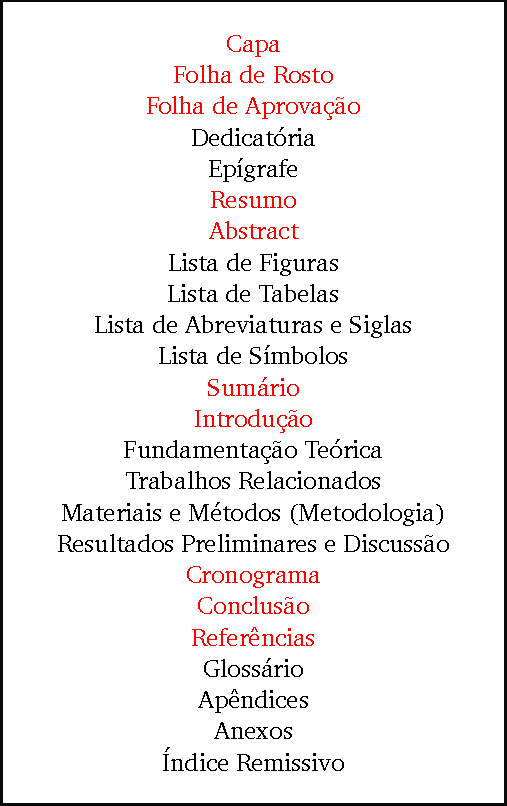
\includegraphics[width=0.5\textwidth]{figuras/estrutura-projeto-qualificacao}
        \label{fig_estrutura_projeto_qualificacao}
    \end{figure}

    Já a \autoref{fig_estrutura_tese_dissertacao} apresenta uma estrutura para uma tese de doutorado ou dissertação de mestrado, conforme a norma \citeonline{NBR14724:2011}.

    Cabe ressaltar que, em todas as figuras, os elementos obrigatórios estão destacados em vermelho, os demais são opcionais.

    \begin{figure}[!htb]
        \centering
        \caption{Estrutura sugerida de uma Tese de Doutorado ou Dissertação de Mestrado}
        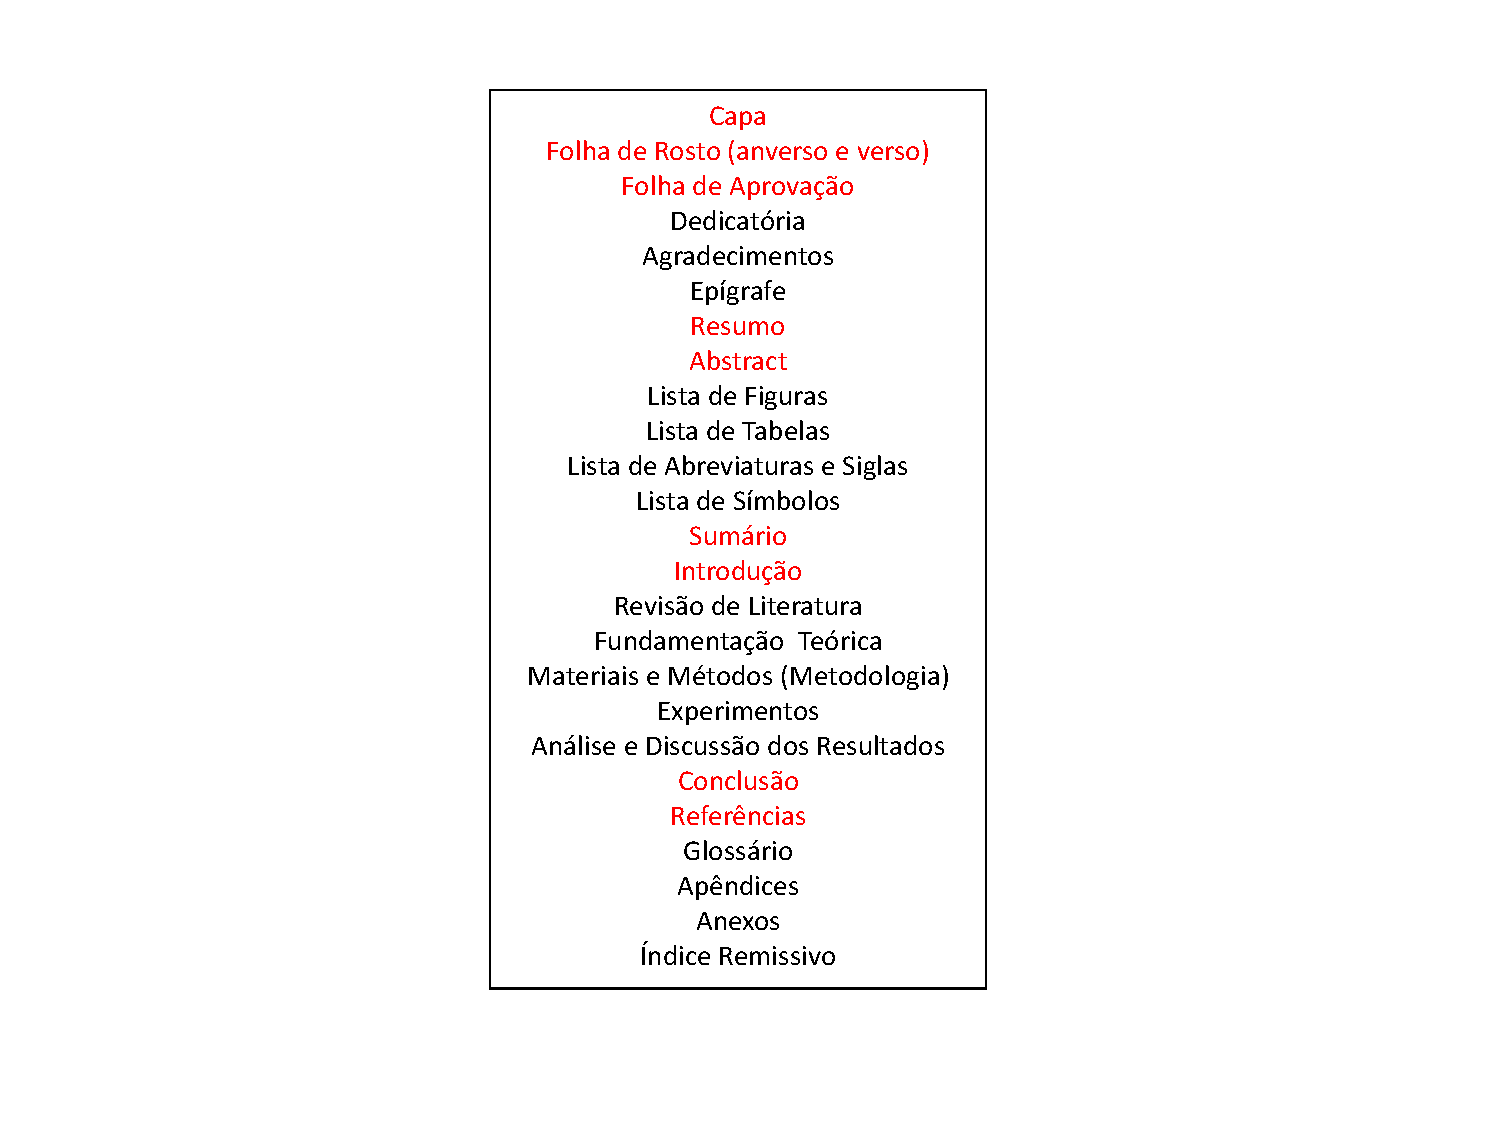
\includegraphics[width=0.5\textwidth]{figuras/estrutura-tese-dissertacao}
        \label{fig_estrutura_tese_dissertacao}
    \end{figure}

    % O comando abaixo adiciona uma quebra de página no documento
    \newpage

    Observe que a estrutura de um projeto de qualificação é muito similar à da tese ou dissertação.
    A única diferença existente é que num projeto de qualificação o autor certamente terá, via de regra, apenas resultados parciais e preliminares.
    Além disso, estando o trabalho ainda em andamento, há que se apresentar um cronograma de trabalho que evidencie que o mesmo poderá ser concluído nos prazos estabelecidos pelo programa.

    Por fim, como foi dito, este \emph{template} pode ser utilizado para outros trabalhos acadêmicos.
    Neste caso, a \autoref{fig_estrutura_projeto_pesquisa} apresenta uma sugestão de projeto de pesquisa a ser submetido ao programa para fins de admissão ao mesmo, conforme a norma \citeonline{NBR15287:2005}.

    \begin{figure}[!htb]
        \centering
        \caption{Estrutura sugerida de um projeto de pesquisa para admissão ao PPGMMC}
        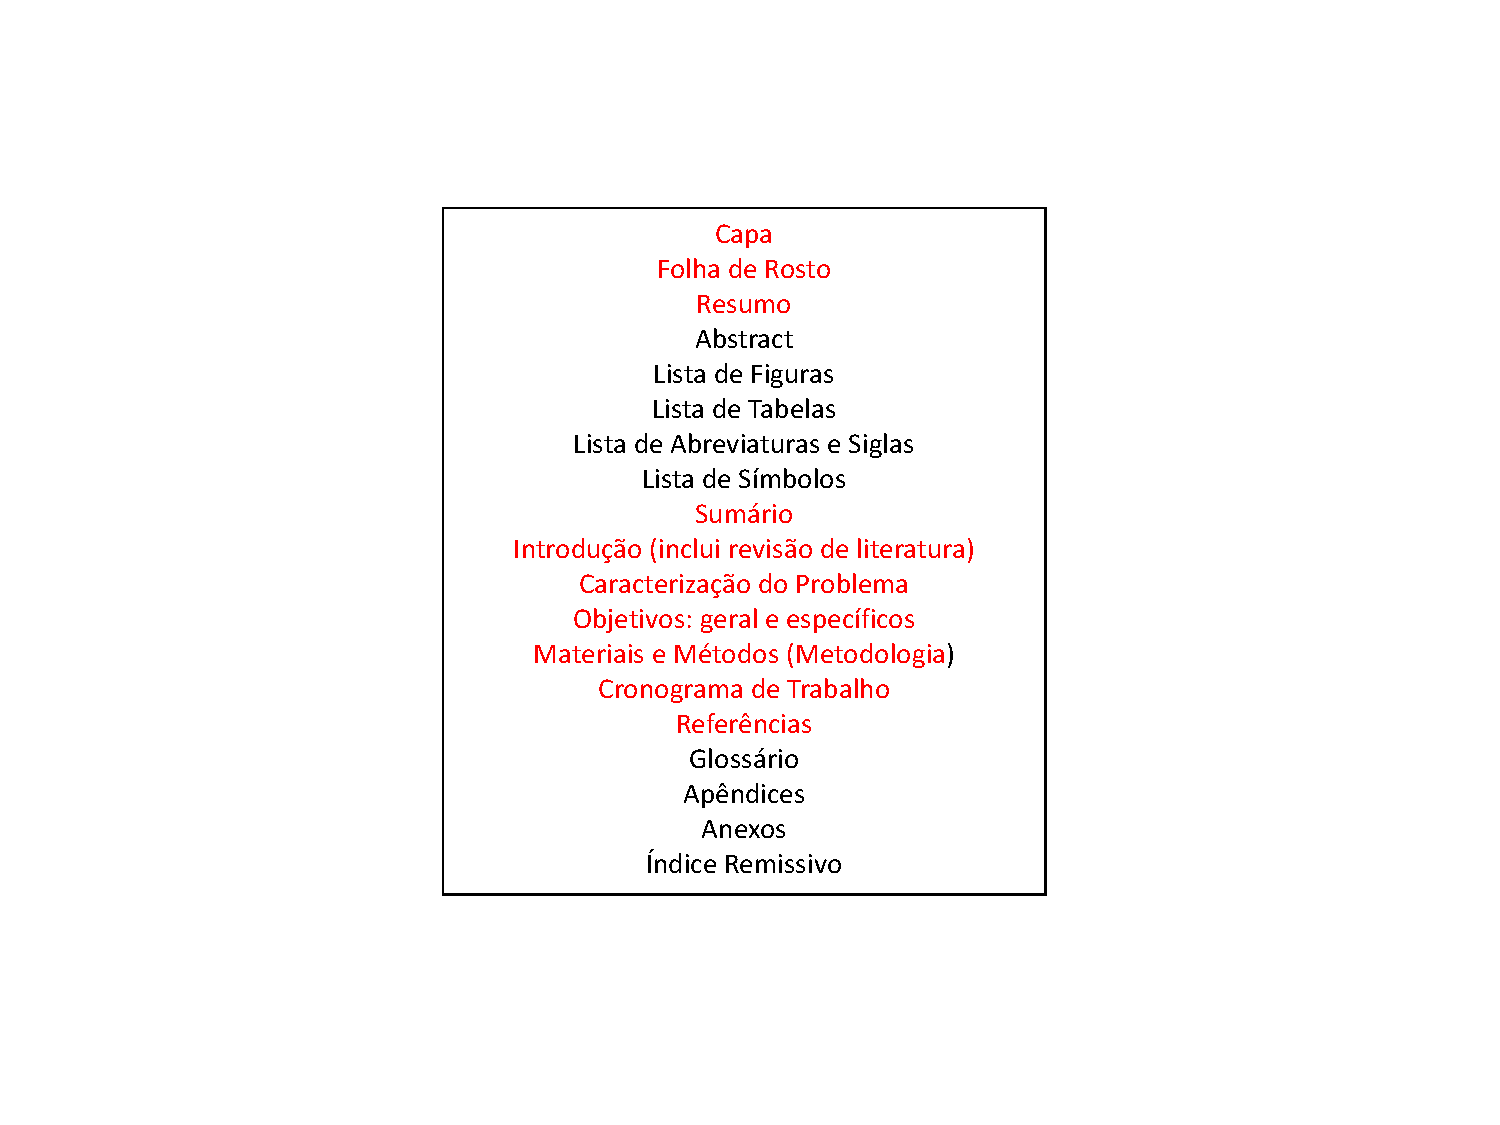
\includegraphics[width=0.6\textwidth]{figuras/estrutura-projeto-pesquisa}
        \label{fig_estrutura_projeto_pesquisa}
    \end{figure}

    Você deverá editar o arquivo principal {\color{red} meu-trabalho.tex} para fazer os ajustes necessários, reiterando que as estruturas apresentadas são meras sugestões.

    A inclusão de reticências (\ldots) no texto deverá ser feita através de um comando especial denominado \verb|\ldots| \cite{LaTeX2014}.
    Assim, esse comando deverá ser utilizado ao invés da digitação de três pontos.

    Para melhor entendimento do uso do estilo de formatação, aconselha-se que o potencial usuário analise os comandos existentes no arquivo {\color{red} meu-trabalho.tex} e os resultados obtidos no arquivo {\color{red} meu-trabalho.pdf}.
    Recomenda-se a consulta ao material de referência do software para a sua correta utilização \cite{Lamport1986,Buerger1989,Kopka2003,Mittelbach2004}.

    % --------------------------------------------------------------------------
    % Novo apêndice
    % --------------------------------------------------------------------------

    \chapter{Sobre as ilustrações}
    \label{chap_sobre_as_ilustracoes}

    A seguir ilustra-se a forma de incluir ilustrações no corpo do texto.
    Pela norma, figuras, tabelas, quadros, equações, quadros, algoritmos, diagrama, etc.
    são tipos específicos de ilustrações.
    As ilustrações (pelo menos alguns tipos específicos) serão indexadas automaticamente em suas respectivas listas.

    A numeração sequencial de figuras, tabelas e equações ocorre de modo automático.

    Referências cruzadas são obtidas através dos comandos \verb|\label{}| e \verb|\ref{}|.
    Por exemplo, não é necessário saber que o número de certo capítulo é \ref{chap_fundamentacao_teorica} para colocar o seu número no texto.
    Alternativamente se pode usar desta forma: \autoref{chap_fundamentacao_teorica}.
    Isto facilita muito a inserção, remoção ou relocação de elementos numerados no texto (fato corriqueiro na escrita e correção de um documento acadêmico) sem a necessidade de enumerá-los todos.

    \section{Figuras}
    \label{sec_figuras}

    A seguir é apresentado um exemplo de figura.
    A \autoref{fig_figura_exemplo} aparece automaticamente na lista de figuras.

    \begin{figure}[!htb]
        \centering
        \caption{Exemplo de figura}
        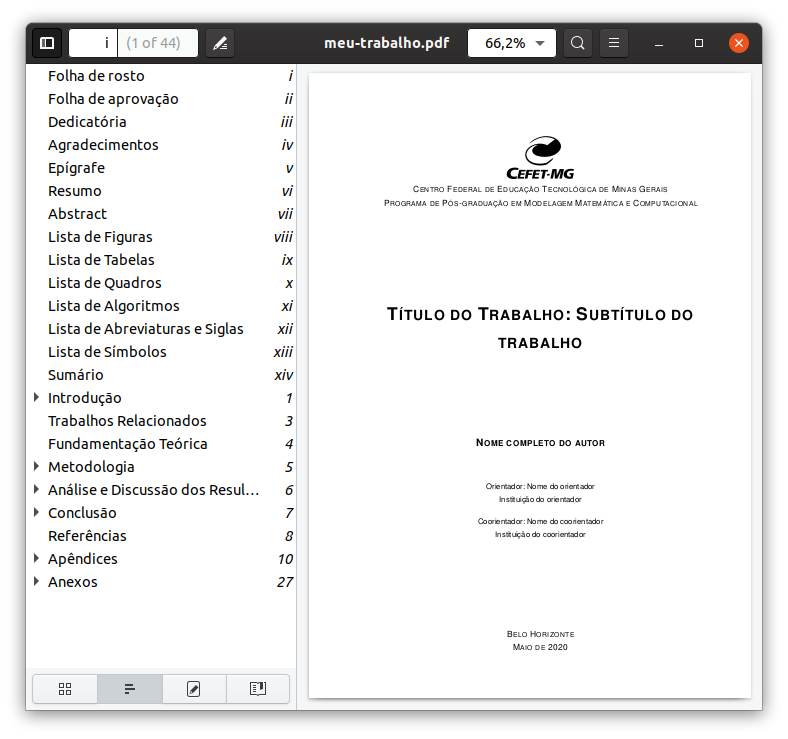
\includegraphics[width=0.75\textwidth]{figuras/figura-exemplo}
        \label{fig_figura_exemplo}
    \end{figure}

    \begin{figure}[!b]
        \centering
        \caption{Exemplo de várias figuras em um único ambiente \textit{figure}.}
        \subtop[][Figura exemplo.]{%
            
\includegraphics[scale=0.2]{figuras/logo-instituicao}%
        }\hspace{2ex} % Ajuste da diagramação
        \subtop[][Figura exemplo.]{%
            
\includegraphics[scale=0.2]{figuras/logo-instituicao}%
        }\hspace{2ex} % Ajuste da diagramação
        \subtop[][Figura exemplo.]{%
            
\includegraphics[scale=0.2]{figuras/logo-instituicao}%
        }
        \label{fig_figura_exemplo2}
    \end{figure}

    \section{Quadros e tabelas}
    \label{sec_tabelas}

    Também é apresentado o exemplo do \autoref{qua_comparabd} e da \autoref{tab_testes}, que aparece automaticamente na lista de quadros e tabelas.

    Informações sobre a construção de tabelas no \LaTeX{} podem ser encontradas na literatura especializada \cite{Lamport1986,Buerger1989,Kopka2003,Mittelbach2004}.

    \begin{quadro}[!htb]
    \centering
    \caption{Hierarquia de restrições das questões.\label{qua:comparabd}}
    \begin{tabular}{|p{7cm}|p{7cm}|}
        \hline
        \textbf{BD Relacionais}                                                                       & \textbf{BD Orientados a Objetos}                  \\
        \hline
        Os dados são passivos, ou seja, certas operações limitadas podem ser automaticamente acionadas quando os dados são usados.
        Os dados são ativos, ou seja, as solicitações fazem com que os objetos executem seus métodos. & Os processos que usam dados mudam constantemente. \\
        \hline
    \end{tabular}
    \fonte{\citeonline{Carvalho2001}}
\end{quadro}


    Muitos confundem, mas existem diferenças entre \index{tabelas} tabelas e \index{quadros} quadros.
    Um quadro é formado por linhas horizontais e verticais, sendo, portanto ``fechado''.
    Você deverá utilizar um quadro quando o conteúdo é majoritariamente não-numérico.
    O número do quadro e o título vem acima do quadro, e a fonte, deve vir abaixo.
    Uma tabela é formada apenas por linhas verticais, sendo, portanto ``aberta''.
    Você deverá utilizar uma tabela quando o conteúdo é majoritariamente numérico.
    O número da tabela e o título vem acima da tabela, e a fonte, deve vir abaixo, tal como no quadro.

    Exemplo de tabela:

    \begin{table}[!htb]
    \centering
    \caption[Resultado dos testes.]{Resultado dos testes.
        \label{tab_testes}}
    \begin{tabular}{rrrrr}
        \toprule
               & Valores 1 & Valores 2 & Valores 3 & Valores 4 \\
        \midrule
        Caso 1 & 0,86      & 0,77      & 0,81      & 163       \\
        Caso 2 & 0,19      & 0,74      & 0,25      & 180       \\
        Caso 3 & 1,00      & 1,00      & 1,00      & 170       \\
        \bottomrule
    \end{tabular}
\end{table}


    % O comando abaixo adiciona uma quebra de página no documento
    \newpage

    \section{Equações}
    \label{sec_equacoes}

    A transformada de Laplace é dada na \autoref{eq_laplace}, enquanto a Eq. \ref{eq_dft} apresenta a formulação da transformada discreta de Fourier bidimensional\footnote{Deve-se reparar na formatação esteticamente perfeita destas equações.}.
    Observe que utilizamos propositalmente duas formas distintas para referenciar as equações.

    \begin{equation}
        X(s) = \int\limits_{t = -\infty}^{\infty} x(t) \, \text{e}^{-st} \, dt
        \label{eq_laplace}
    \end{equation}

    \begin{equation}
        F(u, v) = \sum_{m = 0}^{M - 1} \sum_{n = 0}^{N - 1} f(m, n) \exp \left[ -j 2 \pi \left( \frac{u m}{M} + \frac{v n}{N} \right) \right]
        \label{eq_dft}
    \end{equation}

    \section{Algoritmos}\label{sec_algoritmos}

    Os \index{algoritmos} algoritmos devem ser feitos segundo o \autoref{alg_remocao_aleatoria_vertices}:

    \begin{algorithm}
        \caption{Algoritmo para remoção aleatória de vértices}
        \label{alg_remocao_aleatoria_vertices}
        \KwIn{o número $n$ de vértices a remover, grafo original $G(V, E)$}
        \KwOut{grafo reduzido $G'(V,E)$}
        $removidos \leftarrow 0$ \\
        \While {removidos $<$ n } {
            $v \leftarrow$ Random$(1, ..., k) \in V$ \\
            \For {$u \in adjacentes(v)$} {
                remove aresta (u, v)\\
                $removidos \leftarrow removidos + 1$\\
            }
            \If {há  componentes desconectados} {
                remove os componentes desconectados\\
            }
        }
    \end{algorithm}

    % --------------------------------------------------------------------------
    % Novo apêndice
    % --------------------------------------------------------------------------

    \chapter{Sobre as listas}
    \label{chap_sobre_as_listas}

    O exemplo a seguir ilustra duas listas não numeradas aninhadas, utilizando o ambiente \verb|\itemize|.
    Observe a indentação, bem como a mudança automática do tipo de ``\textit{bullet}'' nas listas aninhadas.

    \begin{itemize}
        \item item não numerado 1
        \item item não numerado 2
              \begin{itemize}
                  \item subitem não numerado 1
                  \item subitem não numerado 2
                  \item subitem não numerado 3
              \end{itemize}
        \item item não numerado 3
    \end{itemize}

    Por outro lado, o exemplo a seguir ilustra duas listas numeradas aninhadas, utilizando o ambiente \verb|\enumerate|.
    Observe a numeração progressiva e indentação das listas aninhadas.

    \begin{enumerate}
        \item item numerado 1
        \item item numerado 2
              \begin{enumerate}
                  \item subitem numerado 1
                  \item subitem numerado 2
                  \item subitem numerado 3
              \end{enumerate}
        \item item numerado 3
    \end{enumerate}

    % --------------------------------------------------------------------------
    % Novo apêndice
    % --------------------------------------------------------------------------

    \chapter{Sobre as citações e chamadas de referências}
    \label{chap_sobre_as_citacoes}

    Citações são trechos transcritos ou informações retiradas das publicações consultadas para a realização do trabalho.
    As citações são utilizadas no texto com o propósito de esclarecer, completar, embasar ou corroborar as ideias do autor.

    Todas as publicações consultadas e efetivamente utilizadas (por citações) devem ser listadas, obrigatoriamente, nas referências bibliográficas, de forma a preservar os direitos autorais e intelectuais.

    A norma ABNT NBR:10520-2002 classifica as citações em: citações livres e citações literais.

    \section{Citações livres}
    \label{sec_citacoes_livres}

    Nas citações livres, reproduzem-se as ideias e informações de um autor, sem, entretanto, ``copiar letra por letra'' o texto do autor.
    Sendo assim, não há muito a dizer sobre como fazer citações livres, exceto que há que se tomar o devido cuidado com o ``recortar e colar e modificar'' para que não se caracterize plágio.

    Quanto à chamada da referência, ela pode ser feita de duas maneiras distintas, conforme o nome do(s) autor(es) façam parte do seu texto ou não.
    Os exemplos a seguir ilustram estas duas possibilidades.

    Enquanto \citeonline{Maturana2003} defendem uma epistemologia baseada na biologia.
    Para os autores, é necessário rever\ldots
    Por outro lado, \citeonline{nunes2017local} contra-argumenta afirmando que\ldots

    As chamadas de referências foram feitas com o comando \verb|\citeonline{}|, que produzirá a formatação correta, conforme a norma ABNT.

    Observe que em ambos os casos anteriores, a frase fica incompleta e incompreensível caso as palavras ``Maturana e Varela'' e ``Barbosa et al.'' não sejam ``pronunciadas''.
    Ou seja, os nomes dos autores fazem parte da frase.
    Neste caso, a formatação automática da chamada de referência coloca os nomes dos autores seguidos, entre parêntesis pelo ano de publicação da obra referenciada.
    Isso apenas no caso em que se usa o esquema autor-ano, que é \textit{padrão} neste modelo \LaTeX{}.

    A segunda maneira de fazer uma chamada de referência deve ser utilizada quando se quer evitar uma interrupção na sequência do texto, o que poderia, eventualmente, prejudicar a leitura.

    % O comando abaixo adiciona uma quebra de página no documento
    \newpage

    Assim, a citação livre é feita e imediatamente após a obra referenciada deve ser colocada entre parênteses.
    Porém, neste caso específico, o nome do autor deve vir em caixa alta, seguido do ano da publicação, como nos exemplos a seguir.

    Há defensores da epistemologia baseada na biologia que argumentam em favor da necessidade de\ldots \cite{Maturana2003}.
    Por outro lado, há os que contra-argumentam afirmando que\ldots  \cite{nunes2017local}.

    Nos dois casos imediatamente acima a chamada de referência deve ser feita com o comando \verb|\cite{chave}|, que produzirá a formatação correta, conforme a norma ABNT.

    Observe que o estilo de redação das frases teve que ser modificado para torná-las compreensíveis sem a menção explícita dos nomes dos autores.
    Estes agora não são parte integrante da frase, ficam entre parêntesis.
    Neste caso, a formatação automática da chamada de referência coloca, entre parêntesis, os nomes dos autores, seguido pelo ano de publicação da obra referenciada.
    Novamente, apenas no caso em que se usa o esquema autor-ano, que é \textit{padrão} neste modelo \LaTeX{}.

    Por fim, cabe chamar a atenção para o detalhe do termo \textit{et al.} que deve ser utilizado quando o trabalho citado possui mais de três autores.
    Esse recurso é automatizado pelo modelo proposto.

    \section{Citações literais}
    \label{sec_citacoes_literais}

    Nas citações literais, reproduzem-se as ideias e informações de um autor, exatamente como este a expressou, ou seja, faz-se uma ``cópia letra por letra'' do texto do autor.
    Sendo assim, obviamente, a obra citada deve ser referenciada, sob pena de se caracterizar plágio.

    Quanto à chamada da referência, ela pode ser feita de qualquer das duas maneiras mencionadas na \autoref{sec_citacoes_livres}, conforme o nome do(s) autor(es) façam parte do seu texto ou não.

    Há duas maneiras distintas de se fazer uma citação literal, conforme o trecho citado seja longo ou curto.

    Quando o trecho citado é longo (4 ou mais linhas) deve-se usar um parágrafo específico para a citação, na forma de um texto recuado (4 cm da margem esquerda), com tamanho de letra menor do aquela utilizada no texto e espaçamento entrelinhas simples.
    Veja o exemplo abaixo.

    \begin{citacao}
        Desse modo, opera-se uma ruptura decisiva entre a reflexividade filosófica, isto é a possibilidade do sujeito de pensar e de refletir, e a objetividade científica.     Encontramo-nos num ponto em que o conhecimento científico está sem consciência.
        Sem consciência moral, sem consciência reflexiva e também subjetiva.
        Cada vez mais o desenvolvimento extraordinário do conhecimento científico vai tornar menos praticável a própria possibilidade de reflexão do sujeito sobre a sua pesquisa \cite[p.~28]{Silva2000}.
    \end{citacao}

    Para se criar o efeito demonstrado na citação anterior, deve-se utilizar o comando:

    \begin{verbatim}
    \begin{citacao}
        <citacao>
    \end{citacao}
\end{verbatim}

    Acima, para a chamada da referência o comando \verb|\cite[p.~28]{Silva2000}| foi utilizado, visto que os nomes dos autores não são parte do trecho citado.

    Observe ainda que foi indicado o número da página da obra citada que contém o trecho citado.
    A localização precisa do trecho citado deve ser indicada sempre, exceto para artigos científicos (tipicamente com poucas páginas, o que geralmente não é o caso de artigos de revisão de literatura) e outros documentos com ``poucas'' páginas.

    Alternativamente, é possível construir uma frase que contenha os autores, e irá encaminhar (por assim dizer) a citação literal.
    Assim sendo, note que após a citação literal não mais aparece o nome dos autores, visto que já se encontra no texto.
    Veja o exemplo seguinte.

    No entanto, \citeonline[p.~33]{Silva2000}, ao fazerem as suas críticas à ciência moderna, afirmam:

    \begin{citacao}
        Mas o curioso é que o conhecimento científico que descobriu os meios realmente extraordinários para, por exemplo, ver aquilo que se passa no nosso sol, para tentar conceber a estrutura das estrelas extremamente distantes, e até mesmo para tentar pesar o universo, o que é algo de extrema utilidade, o conhecimento científico que multiplicou seus meios de observação e de concepção do universo, dos objetos, está completamente cego, se quiser considerar-se apenas a si próprio!
    \end{citacao}

    Já quando o trecho citado é curto (3 ou menos linhas) ele deve ser inserido diretamente no texto entre aspas.
    Veja os dois exemplos seguintes, cada qual utilizando uma forma de chamada de referência.

    A epistemologia baseada na biologia parte do princípio de que ``assumo que não posso fazer referência a entidades independentes de mim para construir meu explicar'' \cite[p.~35]{Maturana2003}.

    A epistemologia baseada na biologia de \citeonline[p.~35]{Maturana2003} parte do princípio de que ``assumo que não posso fazer referência a entidades independentes de mim para construir meu explicar''.

    Finalmente, e isto vale para citações curtas ou longas, caso seja necessário inserir ou suprimir (modificar de modo geral) qualquer palavra ou frase no trecho citado literalmente, isto deve ser feito colocando sua intervenção entre colchetes retos e deve ser indicado explicitamente ao final da citação.
    Veja o exemplo seguinte.

    A epistemologia baseada na biologia parte do princípio de que ``assumo que não posso fazer referência [\textit{sic}] a \underline{entidades independentes} de mim [realidade objetiva] para construir meu explicar'' \cite[p.~35, comentários e grifo nosso]{Maturana2003}.

    \section{Mais detalhes sobre as chamadas de referências}
    \label{sec_chamadas_referencias}

    A seguir há mais exemplos dos comandos para as chamadas de referências e o resultado produzido:

    \citeonline{nunes2017local} $\Longrightarrow$ \verb|\citeonline{nunes2017local}|

    \citeonline[p.~33]{Silva2000} $\Longrightarrow$ \verb|\citeonline[p.~33]{Silva2000}|

    \cite[p.~28]{Silva2000} $\Longrightarrow$ \verb|\cite[p.~28]{Silva2000}|

    \cite[p.~35]{Maturana2003} $\Longrightarrow$ \verb|\cite[p.~35]{Maturana2003}|

    % Espaço vertical
    \vspace{4ex}

    Há que se tomar bastante cuidado com referências cujos autores têm nomes compostos, tipo João de Souza Júnior ou Antônio José da Silva Filho.
    Para que a formatação seja correta, os nomes dos autores no arquivo {\color{red} referencias.bib} deverá ser cadastrado de uma forma específica.

    Os exemplos abaixo ilustram a formatação correta:

    \cite[p.~28]{vanGELDER1998} $\Longrightarrow$ \verb|\cite[p.~28]{vanGELDER1998}|

    \citeonline[p.~28]{vanGELDER1998} $\Longrightarrow$ \verb|\citeonline[p.~28]{vanGELDER1998}|

    % Espaço vertical
    \vspace{4ex}

    Observe ainda o caso em que é feita duas citações juntas \cite{Silva2000, nunes2017local} e como citar endereços de páginas da Internet \cite{IRL2014}.

    % --------------------------------------------------------------------------
    % Novo apêndice
    % --------------------------------------------------------------------------

    \chapter{Sobre as referências bibliográficas}
    \label{chap_sobre_as_referencias_bibliograficas}

    A bibliografia é feita no padrão \textsc{Bib}\TeX{}.
    As referências são colocadas em um arquivo separado chamado {\color{red} referencias.bib}.
    Os elementos de cada item bibliográfico que devem constar nas referências bibliográficas são apresentados a seguir.
    Tais referências bibliográficas devem seguir a norma \citeonline{NBR6023:2002} da ABNT\footnote{As normas técnicas da ABNT não são gratuitas.}.

    \section{Entradas de referências}
    \label{sec_entradas_de_referencias}

    Entradas são objetos de citação bibliográficas.
    Dito de outra forma, são as categorias dos tipos de documentos e materiais componentes da bibliografia.
    A classe abn\TeX{} define as seguintes entradas:

    \begin{verbatim}
        @book
        @inbook
        @article
        @phdthesis
        @mastersthesis
        @monography
        @techreport
        @manual
        @proceedings
        @inproceedings
        @journalpart
        @booklet
        @patent
        @unpublished
        @misc
    \end{verbatim}

    Cada entrada é formatada pelo modelo de uma forma específica.
    Algumas entradas foram introduzidas especificamente para atender à norma \citeonline{NBR6023:2002}, são elas: \verb|@monography|, \verb|@journalpart|,\verb|@patent|.
    As demais entradas são padrão \textsc{Bib}\TeX{}.
    Para maiores detalhes, refira-se a \citeonline{abnTeX22014d}, \citeonline{abnTeX22014b}, \citeonline{abnTeX22014c}.

    A entrada \verb|@monography| é utilizada para cadastrar referências a trabalhos de conclusão de curso, monografias de cursos de especialização (pós-graduação \textit{lato sensu}), e outros trabalhos monográficos, exceto dissertação de mestrado e tese de doutorado.
    Eu particularmente, não considero que a formatação deste tipo de entrada seja adequada.
    Para um trabalho de conclusão de curso (TCC) de curso de graduação, que deveria ser formatado como ``[\ldots] Trabalho de Conclusão de Curso (Bacharelado em Engenharia de Computação) [\ldots]''; no entanto o uso de \verb|@monography| irá produzir ``[\ldots] Monografia (Bacharelado em Engenharia de Computação) [\ldots]''.
    A própria  \citeonline{NBR6023:2002}, na seção 8.11.4, apresenta um exemplo com a formatação diferente daquela proporcionada por \citeonline{abnTeX22014d}.

    A entrada \verb|@journalpart| é utilizada, conforme diz o manual \cite{abnTeX22014d}, para cadastrar referências e formatar partes de periódicos.
    Não fica claro o que se quer dizer com partes de journal.
    Em alguns casos, tais partes são artigos - e portanto, deveriam ser registradas como \verb|@article| - noutros casos, parece serem matérias ou textos em revistas ou jornais (não científicos).
    Salvo melhor juízo, me parece que esta entrada deve ser utilizada apenas neste último contexto.

    A entrada \verb|@patent| é utilizada, obviamente, para cadastrar referências a patentes.

    Todavia, o fato é que a normalização de referências conforme a norma \citeonline{NBR6023:2002} requer que muitos dos campos do \textsc{Bib}\TeX{} sejam adaptados.
    Sendo mais explícito, ao baixar um arquivo {\color{red} .bib} de um trabalho, principalmente se for internacional, e inseri-lo ``\textit{as is}'' em suas referências, há grande chance dessa referência ser formatada de modo errado, no que concerne à norma \citeonline{NBR6023:2002}.
    Isso é especialmente válido em alguns tipos de documentos de largo uso no meio acadêmico afim às áreas de Ciências Exatas, da Terra e Engenharias.

    Diante disso, para evitar erros de formatação, o correto é após baixar o arquivo {\color{red} .bib} de um trabalho, editá-lo com um editor de textos (usando a codificação UTF8), para verificar se os campos descritores que o \textit{publishers} original utilizou são aqueles requeridos pela norma ABNT.

    Neste contexto, e para esta finalidade, nas seções seguintes é apresentado uma série de exemplos, quase todos, utilizados como exemplos na própria norma \citeonline{NBR6023:2002}.
    Para detalhes dos campos utilizados confira o arquivo {\color{red} referencias.bib}.
    Deve-se estar atento para o fato de que o uso de um sistema de gerenciamento de referências para abrir e/ou editar o arquivo {\color{red} referencias.bib}, pode ocultar campos utilizados pela norma ABNT e, por outro lado, exibir campos não utilizados por ela.
    Ou seja, o aplicativo deve ser configurado adequadamente para exibir \textbf{todos os campos}, mesmo os opcionais.

    \section{Notas de rodapé}
    \label{sec_notas_de_rodape}

    A norma \citeonline{NBR10520:2002} classifica as notas de rodapé em duas categorias: notas explicativas\footnote{É o tipo mais comum de notas que destacam, explicam e/ou complementam o que foi dito no corpo do texto, como esta nota de rodapé, por exemplo.} e notas de referências.
    Já as notas de referências, como o próprio nome já indica, são utilizadas para colocar referências e/ou chamadas de referências sob certas condições\footnotemark{}.

    \footnotetext{Outra nota de rodapé.}

    \subsection{Notas de referências: uso de idem, ibidem, opus citatus e outros}
    \label{subsec_notas_de_referencias}

    Como indica o próprio nome, as notas de referências se prestam como recurso auxiliar para referenciação de bibliografia, e seu uso e aplicação são descritos na norma \citeonline{NBR10520:2002}.

    Estes recursos se referem ao uso de certas expressões consagradas para facilitar a elaboração de referências.
    São eles:

    \begin{itemize}
        \item idem = mesmo autor,
        \item ibidem = mesma obra,
        \item opus citatum = obra citada,
        \item locus citatum = no lugar citado,
        \item passim = aqui e alí,
        \item cf = confira,
        \item et sequentia = e sequência.
    \end{itemize}

    Observe que estes recursos não se adéquam para serem utilizados em listas de referências bibliográficas, nem tampouco no corpo do texto.
    Assim, devem ser utilizados apenas nas notas de referência posicionadas no rodapé \cite[p.~6]{abnTeX22014c}, quando se referem a uma referência já feita anteriormente no corpo do texto.
    Ademais, essas expressões fazem sentido apenas quando aplicadas a citações de uma única referência por vez.
    Enfim, trata-se mais de um recurso estilístico do que algo de primeira necessidade, pelo menos para o tipo de documentos usualmente elaborados nas áreas de Ciências Exatas, da Terra e Engenharias.

    Veja o uso desses tipos de expressões nos exemplos seguintes:

    \Ibidem[p.~7]{abnTeX22014c}

    \opcit[p.~9]{abnTeX22014c}

    \passim{abnTeX22014c}

    \cfcite[p.~3]{abnTeX22014b}

    \etseq[p.~6]{abnTeX22014c}

    \section{Datas em referências}
    \label{sec_datas_em_referencias}

    Quando as chamadas de referências são feitas no modelo autor-ano, como é o caso deste modelo, é evidente que o autor e sobretudo o ano adquirem papel de destaque.
    No caso da data de publicação, esta deve sempre estar presente (é elemento essencial) e indicada em algarismos arábicos.

    A norma ABNT não permite o uso de expressões do tipo ``sem data'' (``[s.d]``) para indicar que não se sabe a data de publicação de certa referência bibliográfica.
    Assim sendo, quando a data não puder ser indicada precisamente, deve-se registrar uma data aproximada entre colchetes, conforme descrito a seguir:

    [1971 ou 1972] $\Longrightarrow$ um ano ou outro,

    [1969?] $\Longrightarrow$ ano provável,

    [1973] $\Longrightarrow$ ano certo, não indicada no item,

    [entre 1906 e 1912] $\Longrightarrow$ use intervalos menores de 20 anos,

    [ca. 1960] $\Longrightarrow$ \textit{circa} de\ldots (data aproximada),

    [197-] $\Longrightarrow$ década certa,

    [197-?] $\Longrightarrow$ década provável,

    [18--] $\Longrightarrow$ século certo,

    [18--?] $\Longrightarrow$ século provável.

    \chapter{Ferramentas para Gerenciar a Bibliografia}
    \label{chap_ferramenta_para_gerenciar_a_bibliografia}

    O arquivo {\color{red} referencias.bib} pode ser editado manualmente usando o
    TeXstudio ou com o uso de um editor próprio para arquivos de bibliografia.
    Se você desejar um editor de bibliografia que eu recomendo é o JabRef.
    Além disso, esse programa permite baixar da internet as referências prontas.

    Os arquivos com as referências bibliográficas tem uma formatação rígida e pouco intuitiva, gerando resultados inesperados em muitos casos. Uma forma de evitar erros na digitação desses arquivos é usar um programa específico para esse fim. Uma opção é o JabRef que gerencia as referências de forma simples. Para instalá-lo basta seguir as instruções de sua página
    \begin{center}
        \url{http://www.jabref.org}
    \end{center}

    Como as normas ABNT estão em dissonância com os padrões internacionais,
    o pacote \textit{abntex2cite} cria campos e não reconhecidos pelo automaticamente
    pelo JabRef.
    É possível fazer as edições a mão quando os campos não são reconhecidos,
    porém, pode ser mais simples ajustar as configurações do JabRef para que
    ele siga as especificações necessárias para o \textit{ABsurd Norms for TeX},
    para isso siga os passos descritos na página
    \begin{center}
        \url{https://github.com/abntex/abntex2/wiki/JabRef}
    \end{center}

    \subsection{Problemas com Conversão para Maiúsculas}

    Nas suas entradas que ficam o nos arquivos {\color{red} .bib}
    você deve tomar cuidado especial com a formatação dos acentos,
    especialmente no campo \textit{author} que sempre é convertido para maiúsculas.
    Nesses casos é recomendável utilizar a acentuação original do \LaTeX{}
    usando comandos e não letras acentuadas, como mostra a tabela

    \begin{center}
        \begin{tabular}{clcclcclcclcclccl}
            á & \verb!{\'a}! &  &
            à & \verb!{\`a}! &  &
            â & \verb!{\^a}! &  &
            ã & \verb!{\~a}! &  &
            ç & \verb!{\c c}!
        \end{tabular}
    \end{center}

    Você não precisa formatar toda a sua entrada desta maneira,
    apenas aquelas que vão ser convertidas para maiúsculas.

    \chapter{Exemplos de Equações}
    \label{chap_exemplos_equacoes}

    As experiências acumuladas demonstram que o desenvolvimento contínuo de
    distintas formas de atuação representa uma abertura para a melhoria do
    investimento em reciclagem técnica.

    No entanto, não podemos esquecer que a complexidade dos estudos efetuados nos
    obriga à análise do processo de comunicação.
    \[
        \begin{split}
            x_n & = A \big( \tilde{x}_n + c_1\tilde{x}_{n-1} + c_2\tilde{x}_{n-2} + \dots + c_k\tilde{x}_{n-k} \big) \\
            & + B \big(   \hat{x}_n + c_1  \hat{x}_{n-1} + c_2  \hat{x}_{n-2} + \dots + c_k  \hat{x}_{n-k} \big) \\
            & = 0 \\
        \end{split}
    \]
    Ainda assim, existem dúvidas a respeito de como a contínua expansão de nossa
    atividade maximiza as possibilidades por conta das diversas correntes de
    pensamento.
    \begin{equation}
        \begin{split}
            x_{n+3}^{(1)} & = a_{11}\; x_{n+2}^{(1)}                                                                  \\[2mm]
            & + a_{12} \left( \, a_{21}x_{n+1}^{(1)}+a_{22}x_{n+1}^{(2)}+a_{23}x_{n+1}^{(3)} \, \right) \\[2mm]
            & + a_{13} \left( \, a_{31}x_{n+1}^{(1)}+a_{32}x_{n+1}^{(2)}+a_{33}x_{n+1}^{(3)} \, \right)
        \end{split}
    \end{equation}

    O empenho em analisar o consenso sobre a necessidade de qualificação oferece uma
    interessante oportunidade para verificação do investimento em reciclagem
    técnica.

    \begin{align*}
        f(y_1) & = 0 + 0 + 0 + 0,015 + \dots + 0,09 + 0 = 0,665 \\
        f(y_0) & = 0 + 0 + 0 + 0,035 + \dots + 0,01 + 0 = 0,335
    \end{align*}

    O incentivo ao avanço tecnológico, assim como a consulta aos diversos militantes nos obriga
    à análise das posturas dos órgãos dirigentes com relação às suas atribuições.

    \[
        g(x_i|y_j) = P(X=x_i|Y=y_j) = \frac{g(x_i) f(y_j|x_i)}{\displaystyle\;\sum_{i=1}^{n} g(x_i) f(y_i|x_i)\;}
    \]

    As experiências acumuladas demonstram que a revolução dos costumes
    assume importantes posições no estabelecimento das formas de ação.

    Assim mesmo, a mobilidade dos capitais internacionais cumpre um papel essencial
    na formulação das diversas correntes de pensamento.
    \[ A\cup B \in \mathcal{A} \qquad  \text{e} \qquad  A'\in \mathcal{A} \]
    Utilizando o Teorema de Bayes, temos
    \begin{align*}
        P(F|E) & = \frac{P(E|F)P(F)}{P(E)}                                \\[3mm]
               & = \frac{P(E|F)P(F)}{P(E|F)P(F) + P(E|M)P(M)}             \\[3mm]
               & = \frac{0,3 \times 0,4}{0,3 \times 0,4 + 0,5 \times 0,6} \\[3mm]
               & \approx 28,57\%
    \end{align*}
    Por conseguinte,
    \[
        P(C_{1}|A_{2}) = \frac{P(A_{2}|C_{1})P(C_{1})}{A_{2}}
        = \frac{\frac{1}{2} \times \frac{1}{3}}{\frac{1}{2}}
        = \frac{1}{3}
    \]
    a percepção das dificuldades facilita a criação do levantamento
    das variáveis envolvidas.

    Nunca é demais lembrar o peso e o significado destes
    problemas, visto que a expansão dos mercados mundiais representa uma abertura
    para a melhoria dos modos de operação convencionais. Pensando mais a longo
    prazo, o novo modelo estrutural aqui preconizado faz parte de um processo de
    gerenciamento do sistema de formação de quadros que corresponde às necessidades.
    \[
        \sin \alpha = \frac{\;\text{cateto oposto}\;}{\text{hipotenusa}}
    \]

    Todas estas questões, devidamente ponderadas, levantam dúvidas sobre se o
    aumento do diálogo entre os diferentes setores produtivos maximiza as
    possibilidades por conta das regras de conduta normativas.
    \begin{equation}\label{eq:serie2}
        f(x) = \frac{a_{0}}{2}
        + \sum_{n=1}^{\infty} \Big( a_{n} \cos\frac{n\pi x}{L} + b_{n} \sin\frac{n\pi x}{L} \Big)
    \end{equation}
    Podemos vislumbrar o modo pelo qual a estrutura atual da organização agrega valor ao estabelecimento da gestão inovadora da qual fazemos parte.
    \begin{align*}
        \int_{-\pi}^{\pi} \sin(nx)\cos(mx)\,dx & =\frac{1}{2}\int_{-\pi}^{\pi}\Big(\sin(m+n)x+\sin(m-n)x\Big)\,dx \\[3mm]
                                               & =\frac{1}{2}\int_{-\pi}^{\pi}\Big(\sin(2nx)+\sin(0)\Big)\,dx     \\[3mm]
                                               & =\frac{1}{2}\int_{-\pi}^{\pi}\sin(2nx)\,dx                       \\[3mm]
                                               & =-\left.\frac{1}{2}\frac{\cos(2nx)}{2n}\right|_{-\pi}^{\pi}      \\[3mm]
                                               & =0
    \end{align*}

    A prática cotidiana
    prova que a valorização de fatores subjetivos garante a contribuição de um grupo
    importante na determinação dos índices pretendidos.
    \[
        f(x) = \sum_{n=1}^{\infty} \frac{2(-1)^{n+1}}{n} \sin(nx)
    \]

    Todavia, a competitividade
    nas transações comerciais é uma das consequências de alternativas às soluções
    ortodoxas.

    \[
        f(x) =
        \begin{cases}
            \; 1, & \text{ se }  -\pi \leq x \leq 0 \\
            \; 0, & \text{ se } 0 < x \leq \pi
        \end{cases}
    \]

    O que temos que ter sempre em mente é que o surgimento do comércio
    virtual não pode mais se dissociar das condições financeiras e administrativas
    exigidas.

    \begin{align*}
        1 \!\times\! 2^0 + 1 \!\times\! 2^1 + 1 \!\times\! 2^2 + 0 \!\times\! 2^3 +
        1 \!\times\! 2^4 + 0 \!\times\! 2^5 + 0 \!\times\! 2^6 + 1 \!\times\! 2^7 & =            \\
        1 + 2 + 4 + 0 + 16 + 0 + 0 + 128                                          & = (151)_{10}
    \end{align*}

    Do mesmo modo, o consenso sobre a necessidade de qualificação estende o alcance
    e a importância do fluxo de informações.

    \[
        \int_{-\pi}^{\pi} 2x\sin(nx)\,dx
        = \left.
        \frac{-2x\cos(nx)}{n}
        \right|_{-\pi}^{\pi}
        = \frac{-4\pi(-1)^n}{n}
    \]

    É importante questionar o quanto o
    acompanhamento das preferências de consumo possibilita uma melhor visão global
    dos conhecimentos estratégicos para atingir a excelência.

    \begin{enumerate}[label=\alph*)]
        \item $f(A\cup B)\leq f(A)+f(B)$
        \item $f(B-A)=f(B)-f(A), \quad $se$\quad A\subseteq B$
        \item $f(A)\leq f(B), \quad $se$\quad A\subseteq B \quad$ (Propriedade monótona)
        \item $f(\emptyset)=0$
    \end{enumerate}

    No mundo atual, a
    adoção de políticas descentralizadoras estimula a padronização dos índices
    pretendidos.

    \[
        A = \{a_{1}\} \cup \{a_{2}\} \cup \dots \cup \{a_{k} \}
    \]
    a propriedade aditiva exige que
    \[
        P(A) = \sum_{i=1}^{k} P({a_{i}})
    \]

    A certificação de metodologias que nos auxiliam a lidar com a
    constante divulgação das informações maximiza as possibilidades por conta de
    alternativas às soluções ortodoxas.

    \[
        M \cup N = (T \cap B) \cup (U \cap B)
        \quad
        \Rightarrow
        \quad
        M \cup N = (T \cup U) \cap B
    \]

    Neste sentido, a estrutura atual da organização promove a alavancagem das regras
    de conduta normativas.

    Uma equação em que alguns jogos se baseiam é a chamada ``super equação''

    \[
        r( \varphi )=
        \left [\,
        \vphantom{\begin{array}{c}1\\2\\3\\\end{array}}
        \left|
        \frac{\,\cos\left( \frac{m_1\varphi }{4} \right)\,}{a}
        \right|^{n_2} + \;\;
        \left|
        \frac{\,\sin\left( \frac{m_2\varphi }{4} \right)\,}{b}
        \right|^{n_3}
        \right]^{-\frac{1}{n_1}}
    \]

    A prática cotidiana prova que a expansão dos mercados
    mundiais deve passar por modificações independentemente das posturas dos órgãos
    dirigentes com relação às suas atribuições.

    \[
        \left\| \vec{v} \right\| = \sqrt{ x_{1}^{2} + x_{2}^{2} + \cdots + x_{n}^{2} \,}
    \]

    \[
        \lambda_1 = \frac
        {
            \begin{vmatrix}
                x & x_1 & x_2 \\
                y & y_1 & y_2 \\
                1 & 1   & 1
            \end{vmatrix}
        }
        {\;
            \begin{vmatrix}
                x_1 & x_2 & x_3 \\
                y_1 & y_2 & y_3 \\
                1   & 1   & 1
            \end{vmatrix}
            \;
        }
        = \frac{S_1}{S}
    \]

    As experiências acumuladas
    demonstram que a mobilidade dos capitais internacionais pode nos levar a
    considerar a reestruturação das direções preferenciais no sentido do progresso.

    \[
        \sin x = x - \frac{x^{3}}{3!} + \frac{x^{5}}{5!} + \frac{x^{7}}{7!} + \cdots
    \]
    e ele mostrou que
    \[
        \sin x = \frac{e^{ix}-e^{-ix}}{2i} \quad \text{e} \quad \cos x = \frac {e^{ix} + e^{-ix}}{2}
    \]

    No mundo atual, o início da atividade geral de formação de atitudes ainda não
    demonstrou convincentemente que vai participar na mudança das novas proposições.

    \[
        \hat{A} = \hat{E} \qquad  \hat{B} = \hat{F} \qquad \hat{C} = \hat{G}
    \]
    \[
        \frac{\;\overline{AB}\;}{\;\overline{EF}\;}
        = \frac{\;\overline{BC}\;}{\;\overline{FG}\;}
        = \frac{\;\overline{CA}\;}{\;\overline{GE}\;}
    \]

    É importante questionar o quanto a crescente influência da mídia afeta
    positivamente a correta previsão do fluxo de informações.

    \[
        f(x) = \tan x = \overline{AT}
    \]
    \[
        f(x) = \csc x = \overline{OC}
    \]

    Neste sentido, o
    comprometimento entre as equipes deve passar por modificações independentemente
    das diretrizes de desenvolvimento para o futuro.

    Consideremos as somas parciais

    \begin{align*}
         & s_1 = a_1                   \\
         & s_2 = a_1 + a_2             \\
         & s_3 = a_1 + a_2 + a_3       \\
         & s_4 = a_1 + a_2 + a_3 + a_4
    \end{align*}
    e, em, geral
    \[
        s_n = a_1 + a_2 + a_3 + a_4 + \dots + a_n
        = \sum_{i=1}^{n} a_i
    \]
    Evidentemente, a determinação
    clara de objetivos aponta para a melhoria do processo de comunicação como um
    todo.

\end{apendicesenv}
            % Apêndices
% -----------------------------------------------------------------------------
% Anexos
% -----------------------------------------------------------------------------

\begin{anexosenv}
\partanexos

% -----------------------------------------------------------------------------
% Primeiro anexo
% -----------------------------------------------------------------------------

\chapter{Nome do anexo}
\label{chap:anexo_a}

Lembre-se que a diferença entre apêndice e anexo diz respeito à autoria do texto e/ou material ali colocado.

Caso o material ou texto suplementar ou complementar seja de sua autoria, então ele deverá ser colocado como um apêndice. Porém, caso a autoria seja de terceiros, então o material ou texto deverá ser colocado como anexo.

Caso seja conveniente, podem ser criados outros anexos para o seu trabalho acadêmico. Basta recortar e colar este trecho neste mesmo documento. Lembre-se de alterar o ``label'' do anexo.

Organize seus anexos de modo a que, em cada um deles, haja um único tipo de conteúdo. Isso facilita a leitura e compreensão para o leitor do trabalho. É para ele que você escreve.

\end{anexosenv}
               % Anexos
\printindex                                             % Índice remissivo

\end{document}
